\chapter{Présentation des systèmes Optitrack et ARDrone}

    % ============= Système Optitrack =============
    \section{Système Optitrack}
        Le système Optitrack est un système permettant de détecter des marqueurs infrarouges grâce à un nombre plus ou moins important de caméras infrarouges. Ce système est composé de caméras infrarouges (au minimum 3) reliées à un hub usb lui-même relié à un ordinateur et d'un logiciel de traitement des données nommé Motive. La figure~\ref{fig:systeme_optitrack} présente le système Optitrack, ainsi qu'une caméra infrarouge.

        \begin{figure}[h]
          \centering
          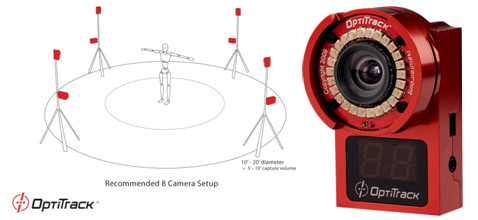
\includegraphics[height=8cm]{images/optitrack_systeme.jpg}
          \caption{Système Optitrack}
          \label{fig:systeme_optitrack}
        \end{figure}

        Ce logiciel permet de calibrer les caméras ensembles, de fixer l'origine du repère par rapport aux caméras, de créer des ``rigidbodies'' à partir de marqueurs infrarouges et d'obtenir la position des différents marqueurs dans l'espace. Il est donc possible de récupérer la position et l'orientation d'un ou plusieurs ``rigidbodies''. \\

        Le logiciel Motive peut fonctionner de façon autonome, mais également en tant que serveur couplé à une autre application. En effet, une application cliente peut se connecter à lui afin de récupérer les informations des marqueurs infrarouges et les utiliser de manière extérieure au logiciel Motive. L'architecture suit celle d'une architecture client-serveur. Pour plus de détails, ce référer à la partie~\ref{sec:prise_en_main_du_systeme_optitrack}.


    % ============= Système ARDrone =============
    \section{Système ARDrone}
        L'ARDrone est un quadricoptère de la marque Parrot. Il est équipé d'un ordinateur ARM 9 cadencé à 468 MHz, d'une RAM de 128 Mo, d'une connectivité Wi-Fi et d'une autonomie de 12 minutes. Il embarque également un accéléromètre 3 axes et un gyroscope 3 axes lui permettant de se stabiliser. La figure~\ref{fig:ardrone} présente un quadricoptère ARDrone.

        \begin{figure}[h]
          \centering
          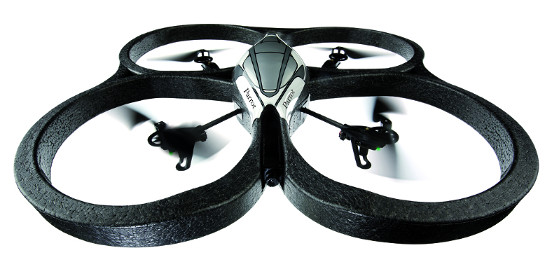
\includegraphics[height=5cm]{images/parrot_ARDrone.jpg}
          \caption{ARDrone}
          \label{fig:ardrone}
        \end{figure}

        Il est par ailleurs équipé de deux caméras, une frontale et une ventrale aidant à sa stabilisation. Bien qu'il embarque un ordinateur, le drone n'est pas nativement programmable. Il n'est que commandable en orientation (yaw), altitude et inclinaison (pitch et roll). Pour plus de détails, ce référer à la partie~\ref{sec:prise_en_main_de_l_ardrone}.
